\documentclass[12pt,oneside]{article}
\usepackage{makeidx,anysize,mflogo,xspace,float,epsfig,url}
\usepackage{amsmath,amsfonts,amssymb,a4wide} 
\usepackage[utf8]{inputenc}
\urlstyle{sf}
\usepackage{hyperref}
\usepackage{graphicx}
\usepackage{graphics}
\usepackage{float}
\usepackage{caption}
\usepackage{colordvi} %??
\usepackage{listings} 
\usepackage{subfigure}
\usepackage{subfloat}
\usepackage{xcolor}
\graphicspath{{./figures/}}
\definecolor{grey}{rgb}{0.95,0.95,0.95}
    \definecolor{red}{rgb}{1.0,0.0,0.0} 
    \definecolor{green}{rgb}{0.0,0.7,0.0}
    \definecolor{blue}{rgb}{0.0,0.0,1.0}
    \lstloadlanguages{bash,Java,C,C++,csh,make,sh}
    \lstset{frame=none,basicstyle=\footnotesize,breaklines,tabsize=2,captionpos=b,
        prebreak={\hbox{$\rightarrow$}},postbreak={\hbox{$\hookrightarrow$}},
        showstringspaces=false,backgroundcolor=\color{grey}\bfseries,
        keywordstyle=\color{blue},commentstyle=\color{green}\textit,
        stringstyle=\color{red}\ttfamily,abovecaptionskip=2pt,aboveskip=0pt,
        belowskip=0pt,belowcaptionskip=0pt,numbers=none,columns=fullflexible, backgroundcolor=\color{grey}}

\begin{document}


\begin{center}
{\bf \Large Pluto: using a sigma-delta audio output} \\ \ \\
G. Goavec-M\'erou, J.-M Friedt \\ \ \\ \today
\end{center}

The investigation of the PlutoSDR hardware, combining an AD9363 radiofrequency frontend
and a Zynq processor, aims at exploiting at best all functionalities of the platform.
In \url{https://www.github.com/oscimp/PlutoSDR/doc} we focused the investigation on the
Zynq by demonstrating the integration of GNU Radio on the processing system (PS) of the
Zynq as provided by the buildroot framework, hence providing a flexible software environment
for exploiting at best the embedded ARM processor. In the current investigation, we focus
on the programmable logic (PL) and aim at demonstrating how to add functionalities to the
FPGA without interfering with the existing AD9363 communication blocks. Interacting with
these blocks will be the topic of another tutorial. In the context of a fully autonomous
commercial broadcast FM radio receiver, we wish to add sound generation capability to the PL
by integrating a sound card capability. The final demonstration will be data acquisition
from the AD9363 using ADi's processing blocks, transfer to the PS in charge of FM demodulation
and sound generation, communication with the kernel module emulating ALSA compatibility, and
sending the resulting audio stream back to the PL embedding the sound card capability. 
Hence, this tutorial aims at extending the previous demonstration of processing the FM signal
on the PS and streaming the resulting audio signal to the computer using the 0MQ framework by
removing the need for the PC acting as a sound card and embedding this audio generation capability
in the PL.

\begin{figure}[h!tb]
\begin{center}
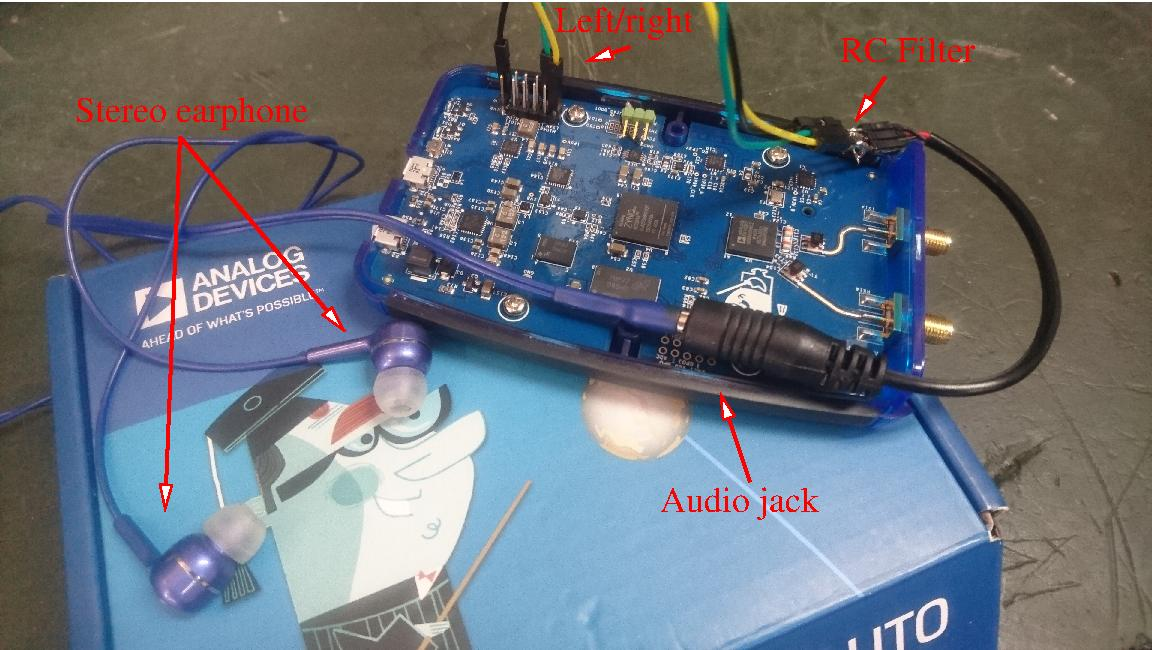
\includegraphics[width=\linewidth]{figures/pluto_audio_ann}
\label{obj}
\end{center}
\caption{Objective of the demonstraiton: convert a PlutoSDR in a fully autonomous FM radio receiver
providing a sound output of the radiofrequency signal demodulated by the PS using GNU Radio processing 
blocks.}
\label{fin}
\end{figure}

Since the PS has no sound controller, the PL design must be adapted to add the IPs needed 
to provided such a functionality. Furthermore, communicating to the IP in charge of sound generation
through the ALSA framework requires updates to the PlutoSDR devicetree describing the hardware 
configuration.

\section{Sound card implementation}

Since no hardware codec is available on the PlutoSDR, we consider using two GPIO connected to the
PL for generating the left and right audio signals.

\subsection{Hardware}

From a hardware perspective, two GPIOs will be toggled by the PL to generate PWM signals. The
PWM to DAC conversion is taken care of by a RC low pass filter bridge connected to each GPIO output
as shown in Fig. \ref{rf_filter}. The resulting voltage can be directly fed to headphones.

\begin{figure}[h!tb]
\center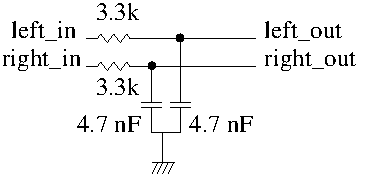
\includegraphics[width=0.5\textwidth]{./figures/RC_filter}
\caption{RC filter with a cutoff frequency of 10.26kHz for converting the $\Sigma\Delta$ output to a smooth
audiofrequency signal driving the headphones.}
\label{rf_filter}
\end{figure}

\subsection{HDL sound card implementation}

The PL will be in charge of toggling the GPIO outputs so that they act as DACs. Such
a result will be achieved by
\begin{itemize}
\item using FIFO based DMA memory to device transfer to collect the samples representing the sound signal
%\ITEm connecting a FIFO to an AXI DMA stream to collect the samples representing the sound signal
\item generate a $\Sigma\Delta$ signal with a mean value equal to the resulting voltage
\item configuring the clock signals to meet the timing requirements expected from standard
sampling rate of sound cards (24, 48 or 96~kHz).
\end{itemize}

Such results are achieved by updating bitstream generated from the various IPs
available on ADi's repository. Modifying the PlutoSDR bitstream provided by
ADi requires first cloning their repository: 
%{\footnotesize
\begin{lstlisting}[language=bash]
git clone https://github.com/analogdevicesinc/hdl     # clone repository
git checkout 401395cdd1980827fd1f7043ce1a10770f666c64 # select hash of current official git
\end{lstlisting}

The original PlutoSDR firmware can always be recovered by {\tt cd projects/pluto} and
{\tt make} from there. Such a synthesis does not require a Vivado license, since the Webpack
is enough for Zynq-7010 support.
%}

To generate the design there are two possibilities:
\begin{enumerate}
\item using the script and the {\tt Makefile} provided in {\tt design} directory.
Such a path requires exporting the \verb!ADI_HDL_DIR! variable to the correct
repository location (see end of this section for pin mapping and bitstream
generation);
\item adding mandatory IPs in an existing PlutoSDR project ({\tt hdl/project/pluto})
\end{enumerate}

Only the latter case requires detailed instructions as given
below. The file {\tt system\_bd.tcl} must be adapted, with:
\begin{lstlisting}[language=TCL]
variable fpga_ip    $::env(OSCIMP_DIGITAL_IP)
# update ip_repo with IPs present in OSCIMP_DIGITAL_IP $
set_property  ip_repo_paths [list ${fpga_ip} ${lib_dirs}] [current_project]
update_ip_catalog
\end{lstlisting}
\noindent
included at the begining of {\tt system\_bd.tcl} to update the list of repositories 
known to Vivado, and

\begin{lstlisting}[language=TCL, numbers=left]
# audio
# axi_deltaSigma needs DMA0 ack/req
ad_ip_parameter sys_ps7 CONFIG.PCW_USE_DMA0 1

# left/right channels
create_bd_port -dir O bit_left_o
create_bd_port -dir O bit_right_o

# clk to generate base time
ad_ip_instance clk_wiz clk_wiz_0

ad_ip_parameter clk_wiz_0 CONFIG.USE_LOCKED false
ad_ip_parameter clk_wiz_0 CONFIG.USE_RESET true
ad_ip_parameter clk_wiz_0 CONFIG.CLKOUT1_REQUESTED_OUT_FREQ 24.576
ad_ip_parameter clk_wiz_0 CONFIG.USE_PHASE_ALIGNMENT false
ad_ip_parameter clk_wiz_0 CONFIG.RESET_TYPE ACTIVE_LOW
ad_ip_parameter clk_wiz_0 CONFIG.PRIM_SOURCE No_buffer

ad_connect clk_wiz_0/clk_in1 sys_ps7/FCLK_CLK0
ad_connect clk_wiz_0/resetn sys_rstgen/peripheral_aresetn

ad_ip_instance axi_deltaSigma axi_deltaSigma
ad_cpu_interconnect 0x43C00000 axi_deltaSigma

ad_connect clk_wiz_0/clk_out1 axi_deltaSigma/data_clk_i
ad_connect bit_right_o axi_deltaSigma/bit_right_o
ad_connect bit_left_o axi_deltaSigma/bit_left_o
ad_connect sys_ps7/FCLK_CLK0 axi_deltaSigma/DMA_REQ_TX_ACLK
ad_connect sys_ps7/FCLK_CLK0 sys_ps7/DMA0_ACLK
ad_connect sys_ps7/DMA0_REQ axi_deltaSigma/dma_req_tx
ad_connect axi_deltaSigma/dma_ack_tx sys_ps7/DMA0_ACK

ad_connect sys_rstgen/peripheral_aresetn axi_deltaSigma/DMA_REQ_TX_RSTN
\end{lstlisting}
appended near the end, to add all functionalities needed for audio output.

Some aspects warrant a more detailed description:
\begin{itemize}
\item in line 3 the PS configuration is modified to enable the Zynq PL330 DMA-controller
control interface. These signals are used for requesting and acknowledging sample 
tranfers through the DMA between the PS memory and the audio controller FIFO, through an
AXI lite bus;
\item in lines 10--17 a {\tt clk\_wiz} is added and configured to generate a
24.576~MHz frequency. This clock is not used for clocking the $\Delta\Sigma$ signal generation 
but to provide a slow clock with a rate, independent of the FPGA clock frequency, multiple of 
commonly used audio frequencies. This is used by a internal prescaler whose maximum value is 
provided by
the driver.
\end{itemize}

Two ports (lines 6--7) were added to the design, for left and right signals, so the constraint 
file ({\tt system\_constr.xdc}) must be updated by adding the associated pin mapping:
\begin{lstlisting} 
# audio
set_property  -dict {PACKAGE_PIN  M12  IOSTANDARD LVCMOS18} [get_ports bit_right_o]
set_property  -dict {PACKAGE_PIN  R10  IOSTANDARD LVCMOS18} [get_ports bit_left_o]
\end{lstlisting} 

\begin{itemize}
\item Pin {\tt M12} corresponds to {\tt L12N} ({\tt PL\_GPIO1}) in connector
silkscreen (Fig. \ref{connector});
\item Pin {\tt R10} corresponds to {\tt L24N} ({\tt PL\_GPIO2}) in connector
silkscreen (Fig. \ref{connector}).
\end{itemize}

\begin{figure}[h!tb]
\begin{center}
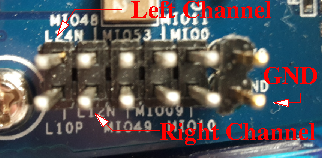
\includegraphics[width=.6\textwidth]{./figures/pluto_gpio_connector.pdf}
\end{center}
\caption{Top left: left channel. Bottom: right channel.}
\label{connector}
\end{figure}

The design is now ready to be synthesized with {\tt make}.

Once the bitstream has been generated, the original PlutoSDR bitstream is overwritten
with the new one using:

\verb|cp pluto.runs/impl_1/system_top.bit /somewhere/PlutoSDR/board/pluto|

\section{Software updates}

\subsection{Buildroot}

According to \url{https://github.com/oscimp/plutosdr}, a buildroot master must
be configured with {\tt zynq\_pluto\_gnuradio\_defconfig}. Since {\tt gr-audio} is
enabled by default, no particular configuration must be done for the buildroot part. 
It is obviously possible to modify the default configuration, through {\tt make
menuconfig} to suppress some package. Since {\tt python} weights about half the
rootfs image size and is mandatory for executing GNU Radio flowgraphs generated using
GNU Radio Companion on the host PC, in addition to GNU Radio SWIG, removing some minor
packages will hardly improve the image size.

\subsection{Linux kernel configuration}

Two modifications must be brought to the kernel configuration. 

First adding some nodes to the devicetree 
({\tt arch/arm/boot/dts/zynq-pluto-sdr-revb.dts}) is needed to add support 
for audio devices. An additional entry must be added to the devicetree part
beginning with \verb|/ {| and finishing with \verb|};|
\begin{lstlisting}[numbers=left]
    audio_clock: audio_clock {
        compatible = "fixed-clock";
        #clock-cells = <0>;
        clock-frequency = <24576000>;
    };

    codec_out: fake_codec {
        #sound-dai-cells = <0>;
        compatible = "ggm,fake_codec";
        clocks = <&audio_clock>;
        clock-names = "mclk";

        status = "okay";
    };

    axi_deltaSigma_0: axi-deltaSigma@43c00000 {
        #sound-dai-cells = <0>;
        compatible = "ggm,axi-deltaSigma";
        reg = <0x43c00000 0x1000>;
        dmas = <&dmac_s 0>;
        dma-names = "tx";
        clocks = <&clkc 15>, <&audio_clock>;
        clock-names = "axi", "ref";
    };

    pluto_sound {
        compatible = "simple-audio-card";
        simple-audio-card,name = "PlutoSDR PWM";
        simple-audio-card,widgets = "Line", "Line Out";
        simple-audio-card,routing = 
            "Line Out", "LOUT",
            "Line Out", "ROUT";

        simple-audio-card,dai-link@0 {
            format = "i2s";
            cpu {
                sound-dai = <&axi_deltaSigma_0>;
                frame-master;
                bitclock-master;
            };
            codec {
                sound-dai = <&codec_out>;
            };
        };
    };
\end{lstlisting}

Again, some details must be provided. According to devicetree rules, the {\tt
.dts} must be a description as close as possible to reality. Hence, the
reference clock frequency is provided by a clock driver ({\tt fixed-clock}).
The node {\tt pluto\_sound} is used to connect the {\tt cpu} part (our IP) and the
{\tt codec} representing the peripheral that converts the numeric format,
provided by CPU, to an analog signal. In the case of the demonstration given later,
a fake driver will be used only because the codec is mandatory.

The second modification focuses on the Linux kernel configuration 
({\tt make linux-menuconfig}) to add audio support and PL330 DMA engine used by
the audio controller, which are not not enabled by default:
{\footnotesize
\begin{verbatim}
Device Drivers -->
    <*>Sound card support -->
        <*>   Advanced Linux Sound Architecture -->
        [...]
        [ ]   ARM sound devices
        [ ]   SPI sound devices
        [ ]   USB sound devices  ----
        <*>   ALSA for SoC audio support  ---> 
            <*>   Audio support for Analog Devices reference designs
            <*>     AXI-I2S support
            <*>   ASoC Simple sound card support
    [*] DMA Engine support  --->
        [...]
        <*>   DMA API Driver for PL330
\end{verbatim}
}

(Analog Devices devices support is only to have access to the PCM DMA engine).

After having modified the {\tt dts} and the kernel configuration, {\tt make linux}
in the Buildroot root directory will compile a new kernel image as well as
device tree binary {\tt .dtb} file including the new functionalities.

\section{Demonstration}

\subsection{GNU Radio Companion generated Python scripts}

The first demonstration of the proper operation of the sound system embedded on the Pluto SDR
relies on a basic sine wave emission on both left and right channels. Using GNU Radio,
a {\tt signal source} configured to generate a sine wave at 1~kHz is connected to an {\tt 
audio sink} (Fig. \ref{signal_to_audio}, top). The result, displayed on an oscilloscope 
(Fig. \ref{signal_to_audio}, bottom) exhibits the proper operation of the processing chain and
hence the compatibility of the sound source embedded in the PL with the Linux ALSA framework.

\begin{figure}[h!tb]
\center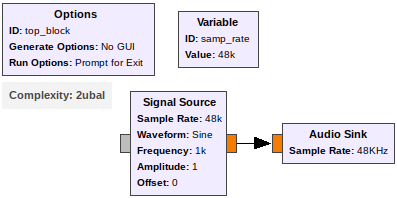
\includegraphics[width=0.7\textwidth]{./figures/pluto_embedded_signal_to_audio}
\center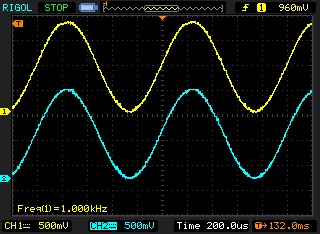
\includegraphics[width=0.7\textwidth]{./figures/signal_to_audio}
\caption{Top: flowgraph generating a 1~kHz signal connected to an audio
sink. Bottom: signal observed and displayed through an oscilloscope}
\label{signal_to_audio}
\end{figure}

A more complex and representative demonstration relies on fetching a radiofrequency
datastream from the AD9363 radiofrequency frontend, transfer the I and Q coefficients
through the PL to the PS, feed the PlutoSDR acquisition block to provide the data
collected at a FM broadcast channel to the WBFM block after low pass filtering and decimating,
and sending the resulting sound signal to the Audio Sink block as demonstrated earlier (Fig. \ref{FM}).

\begin{figure}[h!tb]
\center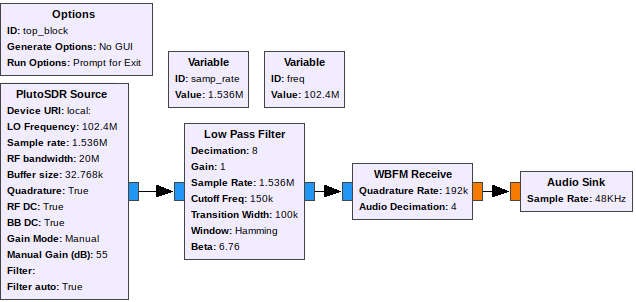
\includegraphics[width=\textwidth]{./figures/pluto_embedded_audio}
\caption{FM broadcast radio signal demodulation on the PlutoSDR PS and playing the resulting
audio signal on the embedded sound card.}
\label{FM}
\end{figure}

\subsection{C++ call to GNU Radio functions}

Python induces a huge footprint on the size of the binary image loaded as RAMdisk. Avoiding 
Python while accessing GNU Radio functionalities is achieved by calling such functions from
C++. As an example of the source to sound card example, the following program allows for generating
the continuous tone without requiring Python on the PS.

\begin{lstlisting}[language=C++]
#include <iostream>
#include <gnuradio/top_block.h>
#include <gnuradio/blocks/file_source.h>
#include <gnuradio/blocks/throttle.h>
#include <gnuradio/analog/sig_source_waveform.h>
#include <gnuradio/analog/sig_source_f.h>
#include <gnuradio/msg_queue.h>
#include <boost/make_shared.hpp>
#include <boost/thread/thread.hpp> //sleep
#include <boost/program_options.hpp>
#include <gnuradio/audio/sink.h>
#include <math.h>

int main(void)
{double samp_rate = 48000;    // audio sampling rate
 gr::top_block_sptr top_block;
 top_block = gr::make_top_block("Acquisition demonstration");
 boost::shared_ptr<gr::analog::sig_source_f> source = gr::analog::sig_source_f::make(samp_rate,
      gr::analog::GR_SIN_WAVE, 1000, 1, 0);
 boost::shared_ptr<gr::audio::sink>audio_sink = gr::audio::sink::make(samp_rate, "", true);
 top_block->connect(source, 0, audio_sink, 0);
 top_block->start(); // Start threads and wait
 printf("Hit any key to stop the application\n");
 getchar();
 top_block->stop();
 top_block->wait();
 return EXIT_SUCCESS;
}
\end{lstlisting}

\end{document}

